% answers.tex —— 2017 年·全国Ⅰ卷·文科 · 参考答案与详细解析片段
% 由 tools/generate_projects.py 依来源总账自 2017/2017_数学真题_文_试题.md + 2017/2017_数学真题_文_解析正文.md + 2017/2017_数学真题_文_答案要点.md 生成，勿手改（改源 MD 后重跑）


\begin{gknotice}
\textbf{ 解析归属声明}：本文解析由本库编写者根据试题\textbf{独立推导}，\textbf{非官方标准答案}。若与官方发布版本不一致，以官方为准。

\textbf{ 卷种提示}：本卷为文理分科时代的旧结构，含\textbf{现已取消}的选做题（第 22/23 题）与\textbf{已删除}的程序框图考点（第 10 题）。

\textbf{重合题说明}：第 4、10 题与第 18(1)、22、23 题与同年理科卷相同，本文给出结论与要点。
\end{gknotice}

\par\medskip

\gkpart{一、选择题}

\begin{answer}
\gksolhead{1}{集合运算}

\textbf{题目}：

已知集合 $A=\{x\mid x<2\}$，$B=\{x\mid3-2x>0\}$，则\mbox{（　　）}

\begin{gkopts}(1)
\task A．$A\cap B=\left\{x\ \middle|\ x<\dfrac32\right\}$
\task B．$A\cap B=\varnothing$
\task C．$A\cup B=\left\{x\ \middle|\ x<\dfrac32\right\}$
\task D．$A\cup B=\mathbf R$
\end{gkopts}

\Needspace{4\baselineskip}
\textbf{解析}

\Needspace{5\baselineskip}
先解 $B$ 中的不等式：

\nopagebreak[4]
\[3-2x>0\ \Longrightarrow\ x<\frac32\]

\Needspace{5\baselineskip}
即 $B=\left\{x\ \middle|\ x<\dfrac32\right\}$。因 $\dfrac32<2$，有 $B\subseteq A$，故

\nopagebreak[4]
\[A\cap B=B=\left\{x\ \middle|\ x<\frac32\right\},\qquad A\cup B=A=\{x\mid x<2\}\]

\gkanswer{答案：A}

\par\medskip

\end{answer}
\begin{answer}
\gksolhead{2}{统计指标的意义}

\textbf{题目}：

为评估一种农作物的种植效果，选了 $n$ 块地作试验田。这 $n$ 块地的亩产量（单位：$\mathrm{kg}$）分别是 $x_1$，$x_2$，$\cdots$，$x_n$，下面给出的指标中可以用来评估这种农作物亩产量\textbf{稳定程度}的是\mbox{（　　）}

\begin{gkopts}(2)
\task A．$x_1,x_2,\cdots,x_n$ 的平均数
\task B．$x_1,x_2,\cdots,x_n$ 的标准差
\task C．$x_1,x_2,\cdots,x_n$ 的最大值
\task D．$x_1,x_2,\cdots,x_n$ 的中位数
\end{gkopts}

\Needspace{4\baselineskip}
\textbf{解析}

四个指标各自刻画的性质：

\begin{center}
\begin{tabular}{ll}
\toprule
指标 & 刻画的性质 \\
\midrule
平均数 & 集中趋势（平均水平） \\
\textbf{标准差} & \textbf{离散程度（波动大小）} \\
最大值 & 极端情况 \\
中位数 & 集中趋势（中间水平） \\
\bottomrule
\end{tabular}
\end{center}

"稳定程度"就是"数据波动是否小"，对应\textbf{标准差}（标准差越小越稳定）。

\gkanswer{答案：B（标准差）}

\par\medskip

\end{answer}
\begin{answer}
\gksolhead{3}{纯虚数}

\textbf{题目}：

下列各式的运算结果为纯虚数的是\mbox{（　　）}

\begin{gkopts}(2)
\task A．$\mathrm i(1+\mathrm i)^{2}$
\task B．$\mathrm i^{2}(1-\mathrm i)$
\task C．$(1+\mathrm i)^{2}$
\task D．$\mathrm i(1+\mathrm i)$
\end{gkopts}

\Needspace{4\baselineskip}
\textbf{解析}

\textbf{先明确定义}：纯虚数是形如 $b\mathrm i\ (b\ne0)$ 的复数，即\textbf{实部为零且虚部不为零}。

逐项计算：

\begin{itemize}
\item \textbf{A}：$\mathrm i(1+\mathrm i)^{2}=\mathrm i\cdot2\mathrm i=2\mathrm i^{2}=-2$ —— 是\textbf{实数}，不是纯虚数；
\item \textbf{B}：$\mathrm i^{2}(1-\mathrm i)=-(1-\mathrm i)=-1+\mathrm i$ —— 实部 $-1\ne0$；
\item \textbf{C}：$(1+\mathrm i)^{2}=1+2\mathrm i+\mathrm i^{2}=2\mathrm i$ —— \textbf{实部为零、虚部为 $2$} 
\item \textbf{D}：$\mathrm i(1+\mathrm i)=\mathrm i+\mathrm i^{2}=-1+\mathrm i$ —— 实部 $-1\ne0$。
\end{itemize}

\begin{gktip}
\textbf{方法提示}：$(1+\mathrm i)^{2}=2\mathrm i$ 与 $(1-\mathrm i)^{2}=-2\mathrm i$ 是复数运算里最常用的两个恒等式，记住可以省下大量展开。

注意 A 项的陷阱：$\mathrm i$ 乘以纯虚数得到的是\textbf{实数}，不是纯虚数。
\end{gktip}

\gkanswer{答案：C（$(1+\mathrm i)^{2}$）}

\par\medskip

\end{answer}
\begin{answer}
\gksolhead{4}{几何概型 · 太极图}

\textbf{题目}：

如图，正方形 $ABCD$ 内的图形来自中国古代的太极图，正方形内切圆中的黑色部分和白色部分关于正方形的中心成中心对称。在正方形内随机取一点，则此点取自黑色部分的概率是\mbox{（　　）}
\nopagebreak[4]
\begin{center}% 2017 全国Ⅰ卷 理2/文4：正方形内的太极图（黑白关于中心成中心对称）
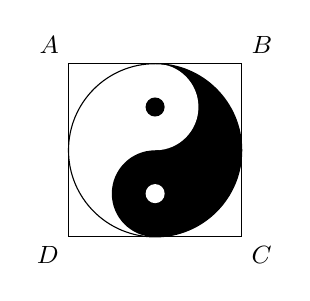
\begin{tikzpicture}[scale=1.1, font=\small]
  % 正方形 ABCD（A 左上、B 右上、C 右下、D 左下），边长 2，内切圆半径 1
  \draw (-1,-1) rectangle (1,1);
  \node[above left]  at (-1, 1) {$A$};
  \node[above right] at ( 1, 1) {$B$};
  \node[below right] at ( 1,-1) {$C$};
  \node[below left]  at (-1,-1) {$D$};
  \begin{scope}
    \clip (0,0) circle (1);
    % 右半黑
    \fill[black] (0,1) arc (90:-90:1) -- cycle;
    % 上小圆白、下小圆黑，构成 S 形分界
    \fill[white] (0,0.5) circle (0.5);
    \fill[black] (0,-0.5) circle (0.5);
    % 鱼眼
    \fill[black] (0,0.5) circle (0.11);
    \fill[white] (0,-0.5) circle (0.11);
  \end{scope}
  \draw (0,0) circle (1);
\end{tikzpicture}
\end{center}
\nopagebreak[4]
\begin{gkopts}(4)
\task A．$\dfrac14$
\task B．$\dfrac\pi8$
\task C．$\dfrac12$
\task D．$\dfrac\pi4$
\end{gkopts}

\textbf{解析}（同理科卷第 2 题）

\Needspace{5\baselineskip}
黑白两部分关于圆心成中心对称 $\Rightarrow$ 面积相等，黑色恰占内切圆的一半。设正方形边长 $2r$：

\nopagebreak[4]
\[P=\frac{\frac12\pi r^{2}}{(2r)^{2}}=\frac\pi8\]

\gkanswer{答案：B（$\dfrac\pi8$）}

\par\medskip

\end{answer}
\begin{answer}
\gksolhead{5}{双曲线通径与三角形面积}

\textbf{题目}：

已知 $F$ 是双曲线 $C:x^{2}-\dfrac{y^{2}}3=1$ 的右焦点，$P$ 是 $C$ 上一点，且 $PF$ 与 $x$ 轴垂直，点 $A$ 的坐标是 $(1,3)$，则 $\triangle APF$ 的面积为\mbox{（　　）}

\begin{gkopts}(4)
\task A．$\dfrac13$
\task B．$\dfrac12$
\task C．$\dfrac23$
\task D．$\dfrac32$
\end{gkopts}

\Needspace{4\baselineskip}
\textbf{解析}

\textbf{第一步：定出 $F$ 和 $P$。}

$a^{2}=1$，$b^{2}=3$，故 $c^{2}=1+3=4$，$c=2$，右焦点 $F(2,0)$。

\Needspace{5\baselineskip}
$PF\perp x$ 轴说明 $P$ 的横坐标也是 $2$。代入双曲线：

\nopagebreak[4]
\[4-\frac{y^{2}}3=1\ \Longrightarrow\ y^{2}=9\ \Longrightarrow\ y=\pm3\]

取 $P(2,3)$（取 $P(2,-3)$ 结果相同）。

\Needspace{5\baselineskip}
\textbf{第二步：算面积。} 把 $PF$ 当作底边（它在竖直线 $x=2$ 上）：

\nopagebreak[4]
\[|PF|=|3-0|=3\]

\Needspace{5\baselineskip}
顶点 $A(1,3)$ 到直线 $x=2$ 的距离为

\nopagebreak[4]
\[d=|1-2|=1\]

\nopagebreak[4]
\[S_{\triangle APF}=\frac12\times3\times1=\frac32\]

\begin{gktip}
\textbf{方法提示}：出现"过焦点且垂直于对称轴的弦"，就是\textbf{通径}，其半长为 $\dfrac{b^{2}}a=\dfrac31=3$ —— 与上面算出的 $|y|=3$ 一致，可以用来快速验算。

选底边时优先选\textbf{竖直或水平的那条}，这样"高"就是坐标差的绝对值，一步可得。
\end{gktip}

\gkanswer{答案：D（$\dfrac32$）}

\par\medskip

\end{answer}
\begin{answer}
\gksolhead{6}{线面平行的判定}

\textbf{题目}：

如图，在下列四个正方体中，$A$，$B$ 为正方体的两个顶点，$M$，$N$，$Q$ 为所在棱的中点，则在这四个正方体中，直线 $AB$ 与平面 $MNQ$ \textbf{不平行}的是\mbox{（　　）}
\nopagebreak[4]
\begin{center}% 2017 全国Ⅰ卷 文6：选项 (A)(B) 的两个正方体
% 前面正方形 (0,0)-(2,2)，后面偏移 (0.85,0.5)；隐藏棱：后左竖棱、左底棱、后底棱
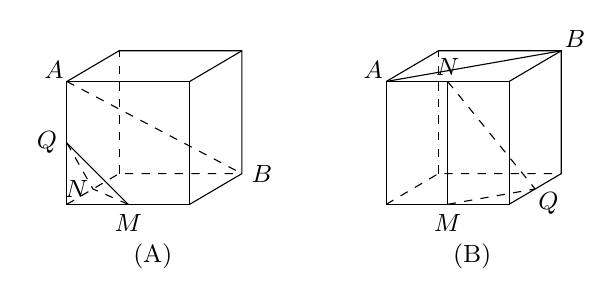
\begin{tikzpicture}[scale=0.78, font=\small]
  % ---------- (A)：A 前左上，B 后右下；M 前下棱中点，N 底面左棱中点，Q 前左竖棱中点 ----------
  \begin{scope}
    \draw (0,0) rectangle (2,2);
    \draw (2,0) -- (2.85,0.5) -- (2.85,2.5) -- (2,2);
    \draw (0,2) -- (0.85,2.5) -- (2.85,2.5);
    \draw[dashed] (0,0) -- (0.85,0.5) -- (2.85,0.5);
    \draw[dashed] (0.85,0.5) -- (0.85,2.5);
    \coordinate (A) at (0,2);
    \coordinate (B) at (2.85,0.5);
    \coordinate (M) at (1,0);
    \coordinate (N) at (0.425,0.25);
    \coordinate (Q) at (0,1);
    \draw[dashed] (A) -- (B);
    \draw (Q) -- (M);
    \draw[dashed] (Q) -- (N) -- (M);
    \node[above left, inner sep=1pt] at (A) {$A$};
    \node[right] at (B) {$B$};
    \node[below] at (M) {$M$};
    \node[left, inner sep=1.5pt] at (N) {$N$};
    \node[left] at (Q) {$Q$};
    \node at (1.4,-0.85) {(A)};
  \end{scope}
  % ---------- (B)：A 前左上，B 后右上；N 前上棱中点，M 前下棱中点，Q 底面右棱中点 ----------
  \begin{scope}[xshift=5.2cm]
    \draw (0,0) rectangle (2,2);
    \draw (2,0) -- (2.85,0.5) -- (2.85,2.5) -- (2,2);
    \draw (0,2) -- (0.85,2.5) -- (2.85,2.5);
    \draw[dashed] (0,0) -- (0.85,0.5) -- (2.85,0.5);
    \draw[dashed] (0.85,0.5) -- (0.85,2.5);
    \coordinate (A) at (0,2);
    \coordinate (B) at (2.85,2.5);
    \coordinate (N) at (1,2);
    \coordinate (M) at (1,0);
    \coordinate (Q) at (2.425,0.25);
    \draw (A) -- (B);
    \draw (N) -- (M);
    \draw[dashed] (N) -- (Q);
    \draw[dashed] (M) -- (Q);
    \node[above left, inner sep=1pt] at (A) {$A$};
    \node[above right, inner sep=1pt] at (B) {$B$};
    \node[above, inner sep=2pt] at (N) {$N$};
    \node[below] at (M) {$M$};
    \node[below right, inner sep=1pt] at (Q) {$Q$};
    \node at (1.4,-0.85) {(B)};
  \end{scope}
\end{tikzpicture}
\end{center}
\nopagebreak[4]
\nopagebreak[4]
\begin{center}% 2017 全国Ⅰ卷 文6：选项 (C)(D) 的两个正方体
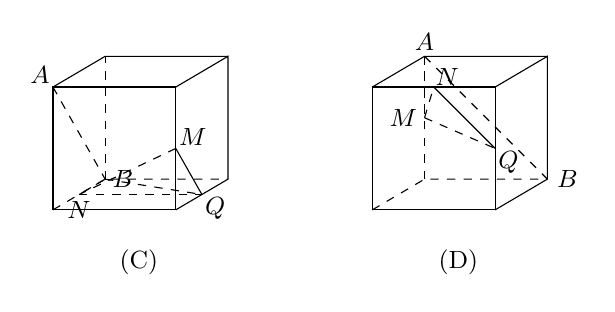
\begin{tikzpicture}[scale=0.78, font=\small]
  % ---------- (C)：A 前左上，B 后左下；M 前右竖棱中点，N 底面左棱中点，Q 底面右棱中点 ----------
  \begin{scope}
    \draw (0,0) rectangle (2,2);
    \draw (2,0) -- (2.85,0.5) -- (2.85,2.5) -- (2,2);
    \draw (0,2) -- (0.85,2.5) -- (2.85,2.5);
    \draw[dashed] (0,0) -- (0.85,0.5) -- (2.85,0.5);
    \draw[dashed] (0.85,0.5) -- (0.85,2.5);
    \coordinate (A) at (0,2);
    \coordinate (B) at (0.85,0.5);
    \coordinate (M) at (2,1);
    \coordinate (N) at (0.425,0.25);
    \coordinate (Q) at (2.425,0.25);
    \draw[dashed] (A) -- (B);
    \draw[dashed] (B) -- (N) (B) -- (Q);   % 到 M N Q 的示意连线在底面/内部
    \draw[dashed] (N) -- (Q);
    \draw (M) -- (Q);
    \draw[dashed] (M) -- (N);
    \node[above left, inner sep=1pt] at (A) {$A$};
    \node[right, inner sep=2.5pt] at (B) {$B$};
    \node[above right, inner sep=1pt] at (M) {$M$};
    \node[below, inner sep=2.5pt] at (N) {$N$};
    \node[below right, inner sep=1pt] at (Q) {$Q$};
    \node at (1.4,-0.85) {(C)};
  \end{scope}
  % ---------- (D)：A 后左上，B 后右下；M 后左竖棱中点，N 前上棱中点，Q 前右竖棱中点 ----------
  \begin{scope}[xshift=5.2cm]
    \draw (0,0) rectangle (2,2);
    \draw (2,0) -- (2.85,0.5) -- (2.85,2.5) -- (2,2);
    \draw (0,2) -- (0.85,2.5) -- (2.85,2.5);
    \draw[dashed] (0,0) -- (0.85,0.5) -- (2.85,0.5);
    \draw[dashed] (0.85,0.5) -- (0.85,2.5);
    \coordinate (A) at (0.85,2.5);
    \coordinate (B) at (2.85,0.5);
    \coordinate (M) at (0.85,1.5);
    \coordinate (N) at (1,2);
    \coordinate (Q) at (2,1);
    \draw[dashed] (A) -- (B);
    \draw[dashed] (A) -- (M);            % A 沿后左竖棱到 M 已被棱覆盖，此线与棱重合
    \draw (N) -- (Q);
    \draw[dashed] (M) -- (N) (M) -- (Q);
    \node[above, inner sep=2pt] at (A) {$A$};
    \node[right] at (B) {$B$};
    \node[left, inner sep=2.5pt] at (M) {$M$};
    \node[above right, inner sep=0.5pt] at (N) {$N$};
    \node[below right, inner sep=1pt] at (Q) {$Q$};
    \node at (1.4,-0.85) {(D)};
  \end{scope}
\end{tikzpicture}
\end{center}
\nopagebreak[4]
\Needspace{4\baselineskip}
\textbf{解析}

\gksubpart{统一坐标系}

\Needspace{5\baselineskip}
四个图的正方体画法一致（前面正对观察者，后面向右上偏移）。设\textbf{棱长为 $2$}，以\textbf{前面左下角}为原点，$x$ 轴向右、$y$ 轴向后、$z$ 轴向上。八个顶点为

\nopagebreak[4]
\[\begin{array}{ll}
\text{\text{前左下}}(0,0,0) & \text{\text{前右下}}(2,0,0)\\
\text{\text{后左下}}(0,2,0) & \text{\text{后右下}}(2,2,0)\\
\text{\text{前左上}}(0,0,2) & \text{\text{前右上}}(2,0,2)\\
\text{\text{后左上}}(0,2,2) & \text{\text{后右上}}(2,2,2)
\end{array}\]

棱长取 $2$ 是为了让所有中点的坐标都是整数。

判定标准：设平面 $MNQ$ 的法向量为 $\boldsymbol n$，

\begin{itemize}
\item $\overrightarrow{AB}\cdot\boldsymbol n=0$ 且 $A\notin$ 平面 $\Rightarrow$ $AB\parallel$ 平面；
\item $\overrightarrow{AB}\cdot\boldsymbol n\ne0$ $\Rightarrow$ $AB$ 与平面\textbf{相交}。
\end{itemize}

\par\medskip

\gksubpart{选项 A：$AB$ 与平面 $MNQ$ 相交（本题答案）}

\Needspace{5\baselineskip}
\textbf{读图定点}：$A$ 是\textbf{前左上}顶点，$B$ 是\textbf{后右下}顶点（图中 $AB$ 为穿过内部的虚线）；$Q$ 是\textbf{前左竖棱}中点，$M$ 是\textbf{前下棱}中点，$N$ 是\textbf{底面左棱}中点。

\nopagebreak[4]
\[A(0,0,2),\quad B(2,2,0),\quad M(1,0,0),\quad N(0,1,0),\quad Q(0,0,1)\]

\nopagebreak[4]
\[\overrightarrow{AB}=(2,2,-2)\ \sim\ (1,1,-1)\]

\Needspace{5\baselineskip}
\textbf{关键观察}：$M$、$N$、$Q$ 分别落在从\textbf{前左下角}出发的三条棱上，且都是中点 —— 这是正方体的"\textbf{截角平面}"，其方程可以直接写出（截距式）：

\nopagebreak[4]
\[\frac x1+\frac y1+\frac z1=1,\qquad\text{\text{即}}\qquad x+y+z=1\]

（验证：$M(1,0,0)$、$N(0,1,0)$、$Q(0,0,1)$ 代入均成立 ）

\Needspace{5\baselineskip}
法向量 $\boldsymbol n=(1,1,1)$。

\nopagebreak[4]
\[\overrightarrow{AB}\cdot\boldsymbol n=1\times1+1\times1+(-1)\times1=1\ne0\]

\textbf{故 $AB$ 与平面 $MNQ$ 相交，不平行。}

\begin{gktip}
\textbf{本质}：平面 $MNQ$ 的法向量 $(1,1,1)$ 恰是\textbf{一条体对角线}的方向，而 $\overrightarrow{AB}=(1,1,-1)$ 是\textbf{另一条体对角线}的方向。正方体的两条体对角线并不垂直（夹角余弦为 $\dfrac13$），所以点积不为零。
\end{gktip}

\par\medskip

\gksubpart{选项 B：$AB\parallel MQ$}

\Needspace{5\baselineskip}
\textbf{读图定点}：$A$ 是\textbf{前左上}顶点，$B$ 是\textbf{后右上}顶点（$AB$ 是顶面的对角线，实线）；$N$ 是\textbf{前上棱}中点，$M$ 是\textbf{前下棱}中点（图中 $MN$ 是前面上的竖直实线），$Q$ 是\textbf{底面右棱}中点。

\nopagebreak[4]
\[A(0,0,2),\quad B(2,2,2),\quad M(1,0,0),\quad N(1,0,2),\quad Q(2,1,0)\]

\nopagebreak[4]
\[\overrightarrow{AB}=(2,2,0),\qquad \overrightarrow{MQ}=(2,1,0)-(1,0,0)=(1,1,0)\]

\nopagebreak[4]
\[\overrightarrow{AB}=2\,\overrightarrow{MQ}\]

\Needspace{5\baselineskip}
\textbf{故 $AB\parallel MQ$}。又 $MQ\subset$ 平面 $MNQ$，而 $A\notin$ 平面（平面方程为 $-x+y+1=0$，代入 $A$ 得 $1\ne0$），由线面平行判定定理：

\nopagebreak[4]
\[AB\parallel\text{\text{平面} }MNQ\]

\par\medskip

\gksubpart{选项 C：$AB\parallel QM$}

\Needspace{5\baselineskip}
\textbf{读图定点}：$A$ 是\textbf{前左上}顶点，$B$ 是\textbf{后左下}顶点；$M$ 是\textbf{前右竖棱}中点，$N$ 是\textbf{底面左棱}中点，$Q$ 是\textbf{底面右棱}中点（图中 $MQ$ 在右侧面上，为实线）。

\nopagebreak[4]
\[A(0,0,2),\quad B(0,2,0),\quad M(2,0,1),\quad N(0,1,0),\quad Q(2,1,0)\]

\nopagebreak[4]
\[\overrightarrow{AB}=(0,2,-2),\qquad \overrightarrow{QM}=(2,0,1)-(2,1,0)=(0,-1,1)\]

\nopagebreak[4]
\[\overrightarrow{AB}=-2\,\overrightarrow{QM}\]

\Needspace{5\baselineskip}
\textbf{故 $AB\parallel QM$}。平面 $MNQ$ 的方程为 $y+z=1$，代入 $A(0,0,2)$ 得 $2\ne1$，$A$ 不在平面内，于是

\nopagebreak[4]
\[AB\parallel\text{\text{平面} }MNQ\]

\par\medskip

\gksubpart{选项 D：$AB\parallel NQ$}

\Needspace{5\baselineskip}
\textbf{读图定点}：$A$ 是\textbf{后左上}顶点，$B$ 是\textbf{后右下}顶点（$AB$ 是后面的对角线，虚线）；$M$ 是\textbf{后左竖棱}中点，$N$ 是\textbf{前上棱}中点，$Q$ 是\textbf{前右竖棱}中点（图中 $NQ$ 在前面上，为实线）。

\nopagebreak[4]
\[A(0,2,2),\quad B(2,2,0),\quad M(0,2,1),\quad N(1,0,2),\quad Q(2,0,1)\]

\nopagebreak[4]
\[\overrightarrow{AB}=(2,0,-2),\qquad \overrightarrow{NQ}=(2,0,1)-(1,0,2)=(1,0,-1)\]

\nopagebreak[4]
\[\overrightarrow{AB}=2\,\overrightarrow{NQ}\]

\Needspace{5\baselineskip}
\textbf{故 $AB\parallel NQ$}。平面 $MNQ$ 的方程为 $x+y+z=3$，代入 $A(0,2,2)$ 得 $4\ne3$，$A$ 不在平面内，于是

\nopagebreak[4]
\[AB\parallel\text{\text{平面} }MNQ\]

\par\medskip

\begin{gktip}
\textbf{方法提示}：

\textbf{1. 找平行线是最快的路。} B、C、D 三个选项中，平面内\textbf{恰好有一条连接两中点的线段直接与 $AB$ 平行}（分别是 $MQ$、$QM$、$NQ$），一眼看出向量成比例就结束了，根本不必求法向量。这也说明命题人是先设计好"哪条中位线平行于 $AB$"，再反推出三个干扰项的。

\textbf{2. 认出"截角平面"就锁定了答案。} 只有 A 图中的 $M$、$N$、$Q$ \textbf{同在从一个顶点出发的三条棱上}，此时平面方程可用截距式直接写成 $x+y+z=1$，法向量是体对角线方向 $(1,1,1)$。考场上看到这个特征就该优先验算 A。

\textbf{3. 平行还需补一句 $A\notin$ 平面。} 若 $\overrightarrow{AB}\cdot\boldsymbol n=0$ 但 $A$ 恰在平面上，那是"直线在平面内"而非平行。本题三个平行选项中 $A$ 都不在平面上，但书写时这一步不能省。

\textbf{4. 棱长设 $2$。} 所有中点坐标都是整数，法向量与点积计算不会出现分数。
\end{gktip}

\gkanswer{答案：A}

\par\medskip

\end{answer}
\begin{answer}
\gksolhead{7}{线性规划}

\textbf{题目}：

设 $x$，$y$ 满足约束条件 $\begin{cases}x+3y\le3\\ x-y\ge1\\ y\ge0\end{cases}$，则 $z=x+y$ 的最大值为\mbox{（　　）}

\begin{gkopts}(4)
\task A．$0$
\task B．$1$
\task C．$2$
\task D．$3$
\end{gkopts}

\Needspace{4\baselineskip}
\textbf{解析}

\textbf{求可行域顶点}：

\begin{itemize}
\item $x+3y=3$ 与 $x-y=1$：由第二式 $x=y+1$，代入第一式 $y+1+3y=3\Rightarrow y=\dfrac12$，$x=\dfrac32$。顶点 $\left(\dfrac32,\dfrac12\right)$；
\item $x+3y=3$ 与 $y=0$：顶点 $(3,0)$；
\item $x-y=1$ 与 $y=0$：顶点 $(1,0)$。
\end{itemize}

\textbf{代入目标函数}：

\begin{center}
\begin{tabular}{cc}
\toprule
顶点 & $z=x+y$ \\
\midrule
$\left(\dfrac32,\dfrac12\right)$ & $2$ \\
$(3,0)$ & $\boxed{3}$ \\
$(1,0)$ & $1$ \\
\bottomrule
\end{tabular}
\end{center}

\gkanswer{答案：D（$3$）}

\par\medskip

\end{answer}
\begin{answer}
\gksolhead{8}{函数图象辨识}

\textbf{题目}：

函数 $y=\dfrac{\sin2x}{1-\cos x}$ 的部分图象大致为\mbox{（　　）}
\nopagebreak[4]
\begin{center}% 2017 全国Ⅰ卷 文8：y=sin2x/(1-cos x) 图象四选一（正确项 C）
% 全部四个面板均由解析式精确绘制：C=g(x)、A=-g(x)、B=g(|x|)、D=-g(|x|)
% （干扰项表达式为重绘构造，原卷为定性示意图）
\begin{tikzpicture}[font=\footnotesize]
\pgfplotsset{
  panel/.style={width=4.6cm, height=3.8cm, axis lines=middle,
    xmin=-3.6, xmax=3.6, ymin=-3.4, ymax=3.4,
    xtick={-3.14159,1,3.14159}, xticklabels={$-\pi$,$1$,$\pi$},
    ytick={1}, yticklabels={$1$},
    xlabel={$x$}, ylabel={$y$},
    every axis x label/.style={at={(current axis.right of origin)}, anchor=west},
    every axis y label/.style={at={(current axis.above origin)}, anchor=south}}}
  \begin{axis}[panel, at={(0,0)}, name=axA]
    \addplot[domain=0.36:3.14159, samples=150, thick] {-sin(deg(2*x))/(1-cos(deg(x)))};
    \addplot[domain=-3.14159:-0.36, samples=150, thick] {-sin(deg(2*x))/(1-cos(deg(x)))};
    \node[below left] at (axis cs:0,0) {$O$};
  \end{axis}
  \node[below=0.5mm] at (axA.south) {(A)};
  \begin{axis}[panel, at={(5.5cm,0)}, name=axB]
    \addplot[domain=0.36:3.14159, samples=150, thick] {sin(deg(2*abs(x)))/(1-cos(deg(x)))};
    \addplot[domain=-3.14159:-0.36, samples=150, thick] {sin(deg(2*abs(x)))/(1-cos(deg(x)))};
    \node[below left] at (axis cs:0,0) {$O$};
  \end{axis}
  \node[below=0.5mm] at (axB.south) {(B)};
  \begin{axis}[panel, at={(0,-4.9cm)}, name=axC]
    \addplot[domain=0.36:3.14159, samples=150, thick] {sin(deg(2*x))/(1-cos(deg(x)))};
    \addplot[domain=-3.14159:-0.36, samples=150, thick] {sin(deg(2*x))/(1-cos(deg(x)))};
    \node[below left] at (axis cs:0,0) {$O$};
  \end{axis}
  \node[below=0.5mm] at (axC.south) {(C)};
  \begin{axis}[panel, at={(5.5cm,-4.9cm)}, name=axD]
    \addplot[domain=0.36:3.14159, samples=150, thick] {-sin(deg(2*abs(x)))/(1-cos(deg(x)))};
    \addplot[domain=-3.14159:-0.36, samples=150, thick] {-sin(deg(2*abs(x)))/(1-cos(deg(x)))};
    \node[below left] at (axis cs:0,0) {$O$};
  \end{axis}
  \node[below=0.5mm] at (axD.south) {(D)};
\end{tikzpicture}
\end{center}
\nopagebreak[4]
\Needspace{4\baselineskip}
\textbf{解析}

\textbf{第一步：定义域与奇偶性。}

\Needspace{5\baselineskip}
分母 $1-\cos x\ne0$，故 $x\ne2k\pi$，即 $x=0$ 处\textbf{没有定义}。

\nopagebreak[4]
\[f(-x)=\frac{\sin(-2x)}{1-\cos(-x)}=\frac{-\sin2x}{1-\cos x}=-f(x)\]

是\textbf{奇函数}，图象关于原点对称。选项 B 呈左右对称（偶函数）形状，\textbf{排除 B}。

\textbf{第二步：考察 $x\to0$ 时的极限}（这是本题最关键的一步）。

\Needspace{5\baselineskip}
当 $x\to0$ 时用等价无穷小：$\sin2x\approx2x$，$1-\cos x\approx\dfrac{x^{2}}2$，于是

\nopagebreak[4]
\[f(x)\approx\frac{2x}{\frac{x^{2}}2}=\frac4x\]

\begin{itemize}
\item $x\to0^{+}$：$f(x)\to+\infty$；
\item $x\to0^{-}$：$f(x)\to-\infty$。
\end{itemize}

选项 A 恰好相反（左侧冲向 $+\infty$、右侧从 $-\infty$ 上来），\textbf{排除 A}。

\textbf{第三步：确定 $(0,\pi)$ 上的符号，区分 C 与 D。}

在 $(0,\pi)$ 上分母 $1-\cos x>0$，故 $f$ 的符号与 $\sin2x$ 相同：

\begin{itemize}
\item $x\in\left(0,\dfrac\pi2\right)$：$2x\in(0,\pi)$，$\sin2x>0$，故 $f>0$；
\item $x=\dfrac\pi2$：$f=0$；
\item $x\in\left(\dfrac\pi2,\pi\right)$：$2x\in(\pi,2\pi)$，$\sin2x<0$，故 $f<0$，\textbf{一直保持为负到 $x=\pi$}；
\item $x=\pi$：$f(\pi)=\dfrac{\sin2\pi}{1-\cos\pi}=\dfrac02=0$。
\end{itemize}

也就是说，在 $\left(\dfrac\pi2,\pi\right)$ 上图象\textbf{全部位于 $x$ 轴下方}，直到 $x=\pi$ 才回到 $x$ 轴。选项 D 在接近 $\pi$ 处又穿回 $x$ 轴上方，\textbf{排除 D}。

\begin{gktip}
\textbf{方法提示}：函数图象题的通用四步是"\textbf{定义域 → 奇偶性 → 特殊点/极限 → 局部符号}"。本题的分水岭在第二步：$1-\cos x$ 在 $x\to0$ 时是\textbf{二阶}无穷小（$\sim\dfrac{x^{2}}2$），而分子是\textbf{一阶}的，所以商发散到无穷 —— 若误以为分子分母同阶而算出有限极限，四个图就全都区分不开了。

化简技巧：$\dfrac{\sin2x}{1-\cos x}=\dfrac{2\sin x\cos x}{1-\cos x}$，也可用半角公式写成 $\dfrac{4\cos^{2}\frac x2\cos x}{\ }\cdots$，但对本题而言直接用等价无穷小最快。
\end{gktip}

\gkanswer{答案：C}

\par\medskip

\end{answer}
\begin{answer}
\gksolhead{9}{对数函数的对称性}

\textbf{题目}：

已知函数 $f(x)=\ln x+\ln(2-x)$，则\mbox{（　　）}

\begin{gkopts}(2)
\task A．$f(x)$ 在 $(0,2)$ 单调递增
\task B．$f(x)$ 在 $(0,2)$ 单调递减
\task C．$y=f(x)$ 的图象关于直线 $x=1$ 对称
\task D．$y=f(x)$ 的图象关于点 $(1,0)$ 对称
\end{gkopts}

\Needspace{4\baselineskip}
\textbf{解析}

\Needspace{5\baselineskip}
\textbf{第一步：定义域。} 需要 $x>0$ 且 $2-x>0$，故

\nopagebreak[4]
\[x\in(0,2)\]

\Needspace{5\baselineskip}
\textbf{第二步：合并对数。} 在定义域内两个真数都为正，可以合并：

\nopagebreak[4]
\[f(x)=\ln\left[x(2-x)\right]\]

\Needspace{5\baselineskip}
\textbf{第三步：分析内层函数。} 记

\nopagebreak[4]
\[u(x)=x(2-x)=-x^{2}+2x=-(x-1)^{2}+1\]

这是开口向下、顶点在 $x=1$ 的抛物线，\textbf{关于直线 $x=1$ 对称}，且在 $(0,1)$ 递增、$(1,2)$ 递减。

\textbf{第四步：结论。} $\ln$ 是单调递增函数，复合后：

\begin{itemize}
\item $f$ 在 $(0,1)$ 递增、在 $(1,2)$ 递减 —— 所以 \textbf{A、B 都错}（$f$ 在 $(0,2)$ 上不单调）；
\item $u$ 关于 $x=1$ 对称 $\Rightarrow$ $f$ 也关于 $x=1$ 对称（因为 $u(1+t)=u(1-t)$ 直接给出 $f(1+t)=f(1-t)$）—— \textbf{C 正确}；
\item 关于点 $(1,0)$ 对称要求 $f(1+t)+f(1-t)=0$，但实际上 $f(1+t)=f(1-t)$，两者之和为 $2f(1+t)=2\ln u\ne0$（例如 $t=0$ 时和为 $2\ln1\cdot2=0$？验证：$f(1)=\ln1=0$，$2f(1)=0$；但取 $t=0.5$：$f(1.5)=\ln(1.5\times0.5)=\ln0.75\ne0$，故 $f(1.5)+f(0.5)=2\ln0.75\ne0$）—— \textbf{D 错}。
\end{itemize}

\begin{gktip}
\textbf{方法提示}：见到两个对数相加，\textbf{第一动作是在定义域内合并成一个对数}，问题立刻从"两个函数的和"变成"一个二次函数的复合"，所有性质都由内层二次函数决定。

判断"关于直线对称"用 $f(a+t)=f(a-t)$，判断"关于点 $(a,b)$ 对称"用 $f(a+t)+f(a-t)=2b$ —— 这两个式子要分清。
\end{gktip}

\gkanswer{答案：C（图象关于直线 $x=1$ 对称）}

\par\medskip

\end{answer}
\begin{answer}
\gksolhead{10}{程序框图}

\textbf{题目}：

如图程序框图是为了求出满足 $3^{n}-2^{n}>1000$ 的最小偶数 $n$，那么在 $\Diamond$ 和 $\square$ 两个空白框中，可以分别填入\mbox{（　　）}
\nopagebreak[4]
\begin{center}% 2017 全国Ⅰ卷 理8/文10：求满足 3^n-2^n>1000 的最小偶数 n 的程序框图
% 两个空白框（菱形与左侧矩形）是题目要求填入的位置，故留白
\begin{tikzpicture}[font=\small, >=Stealth, node distance=8mm,
  box/.style={draw, minimum height=1.9em, inner xsep=7pt},
  term/.style={draw, rounded corners=7pt, minimum height=1.9em, inner xsep=9pt},
  io/.style={draw, trapezium, trapezium left angle=70, trapezium right angle=110,
             minimum height=1.9em, inner xsep=2pt},
  dec/.style={draw, diamond, aspect=2.4, inner sep=1.5pt}]
  \node[term] (start) {开始};
  \node[io, below=of start] (in) {输入 $n=0$};
  \coordinate[below=5mm of in] (merge);
  \node[box, below=2mm of merge] (calc) {$A=3^{n}-2^{n}$};
  \node[dec, below=of calc] (cond) {\phantom{$A\le1000$}};
  \node[box, left=12mm of calc, minimum width=5.2em] (blank) {\phantom{$n=n+2$}};
  \node[io, below=of cond] (out) {输出 $n$};
  \node[term, below=of out] (end) {结束};
  \draw[->] (start) -- (in);
  \draw[->] (in) -- (calc);
  \draw[->] (calc) -- (cond);
  \draw[->] (cond) -- node[right]{否} (out);
  \draw[->] (out) -- (end);
  \draw[->] (cond) -| node[below, pos=0.18]{是} (blank);
  \draw[->] (blank) |- (merge);
\end{tikzpicture}
\end{center}
\nopagebreak[4]
\begin{gkopts}(2)
\task A．$A>1000$ 和 $n=n+1$
\task B．$A>1000$ 和 $n=n+2$
\task C．$A\le1000$ 和 $n=n+1$
\task D．$A\le1000$ 和 $n=n+2$
\end{gkopts}

\begin{gktip}
\textbf{注}：程序框图（算法初步）在现行新课标中已删除。
\end{gktip}

\Needspace{0.25\textheight}

\textbf{解析}（同理科卷第 8 题）

框图中菱形的"\textbf{是}"分支指回循环体，故其中填的是"尚未达标、需要继续"的条件 $A\le1000$；要找最小\textbf{偶数}，初值 $n=0$，步长应为 $2$。

验证：$n=2$ 时 $A=5$；$n=4$ 时 $A=65$；$n=6$ 时 $A=665$；$n=8$ 时 $A=6305>1000$，输出 $8$ 

\gkanswer{答案：D（$A\le1000$ 和 $n=n+2$）}

\par\medskip

\end{answer}
\begin{answer}
\gksolhead{11}{解三角形}

\textbf{题目}：

$\triangle ABC$ 的内角 $A$，$B$，$C$ 的对边分别为 $a$，$b$，$c$，已知 $\sin B+\sin A(\sin C-\cos C)=0$，$a=2$，$c=\sqrt2$，则 $C=$\mbox{（　　）}

\begin{gkopts}(4)
\task A．$\dfrac\pi{12}$
\task B．$\dfrac\pi6$
\task C．$\dfrac\pi4$
\task D．$\dfrac\pi3$
\end{gkopts}

\Needspace{4\baselineskip}
\textbf{解析}

\Needspace{5\baselineskip}
\textbf{第一步：消掉 $B$。} 三角形中 $B=\pi-(A+C)$，故

\nopagebreak[4]
\[\sin B=\sin(A+C)=\sin A\cos C+\cos A\sin C\]

\Needspace{5\baselineskip}
代入条件式：

\nopagebreak[4]
\[\underbrace{\sin A\cos C}_{}+\cos A\sin C+\sin A\sin C-\underbrace{\sin A\cos C}_{}=0\]

\Needspace{5\baselineskip}
\textbf{首尾两项恰好抵消}：

\nopagebreak[4]
\[\cos A\sin C+\sin A\sin C=0\ \Longrightarrow\ \sin C\left(\sin A+\cos A\right)=0\]

\Needspace{5\baselineskip}
\textbf{第二步：定 $A$。} 因 $C\in(0,\pi)$，$\sin C\ne0$，故

\nopagebreak[4]
\[\sin A+\cos A=0\ \Longrightarrow\ \tan A=-1\ \Longrightarrow\ A=\frac{3\pi}4\]

（$A\in(0,\pi)$ 中只有这一个解。）

\Needspace{5\baselineskip}
\textbf{第三步：用正弦定理求 $C$。}

\nopagebreak[4]
\[\frac a{\sin A}=\frac c{\sin C}\ \Longrightarrow\ \frac2{\frac{\sqrt2}2}=\frac{\sqrt2}{\sin C}\ \Longrightarrow\ 2\sqrt2=\frac{\sqrt2}{\sin C}\]

\nopagebreak[4]
\[\sin C=\frac12\]

\Needspace{5\baselineskip}
\textbf{第四步：舍根。} $\sin C=\dfrac12$ 对应 $C=\dfrac\pi6$ 或 $C=\dfrac{5\pi}6$。但 $A=\dfrac{3\pi}4$ 已是钝角，一个三角形不能有两个钝角，且 $A+C<\pi$ 要求 $C<\dfrac\pi4$，故

\nopagebreak[4]
\[C=\frac\pi6\]

\begin{gktip}
\textbf{方法提示}：条件式里同时出现 $\sin B$ 与 $A$、$C$ 的三角函数，\textbf{必然要用 $B=\pi-(A+C)$ 把 $B$ 消掉}。展开后 $\sin A\cos C$ 抵消是本题的设计巧思 —— 若展开后没有出现抵消，多半是展开写错了，可以据此自查。

最后的舍根不能省：\textbf{已经确定 $A$ 是钝角，就意味着另外两角必为锐角}。
\end{gktip}

\gkanswer{答案：B（$\dfrac\pi6$）}

\par\medskip

\end{answer}
\begin{answer}
\gksolhead{12}{椭圆上的张角}

\textbf{题目}：

设 $A$，$B$ 是椭圆 $C:\dfrac{x^{2}}3+\dfrac{y^{2}}m=1$ 长轴的两个端点。若 $C$ 上存在点 $M$ 满足 $\angle AMB=120^\circ$，则 $m$ 的取值范围是\mbox{（　　）}

\begin{gkopts}(2)
\task A．$(0,1]\cup[9,+\infty)$
\task B．$\left(0,\sqrt3\right]\cup[9,+\infty)$
\task C．$(0,1]\cup[4,+\infty)$
\task D．$\left(0,\sqrt3\right]\cup[4,+\infty)$
\end{gkopts}

\Needspace{4\baselineskip}
\textbf{解析}

\textbf{核心结论}：对椭圆长轴的两个端点 $A$、$B$，椭圆上动点 $M$ 对 $AB$ 的张角 $\angle AMB$ 在 \textbf{$M$ 位于短轴端点时取得最大值}。

（直观理解：$M$ 越靠近长轴端点，张角越接近 $0$；越远离长轴，张角越大。）

因此"存在 $M$ 使 $\angle AMB=120^\circ$"等价于"\textbf{最大张角 $\ge120^\circ$}"。

\textbf{情形一：长轴在 $x$ 轴上}，即 $0<m<3$。

此时 $a=\sqrt3$（半长轴），$b=\sqrt m$（半短轴），$A\left(-\sqrt3,0\right)$，$B\left(\sqrt3,0\right)$，短轴端点 $M_0\left(0,\sqrt m\right)$。

\Needspace{5\baselineskip}
$\triangle AM_0B$ 是等腰三角形，半顶角满足

\nopagebreak[4]
\[\tan\frac{\angle AM_0B}2=\frac{\sqrt3}{\sqrt m}\]

\Needspace{5\baselineskip}
要求 $\angle AM_0B\ge120^\circ$，即半顶角 $\ge60^\circ$：

\nopagebreak[4]
\[\frac{\sqrt3}{\sqrt m}\ge\tan60^\circ=\sqrt3\ \Longrightarrow\ \sqrt m\le1\ \Longrightarrow\ m\le1\]

\Needspace{5\baselineskip}
结合 $0<m<3$：

\nopagebreak[4]
\[0<m\le1\]

\Needspace{0.25\textheight}

\textbf{情形二：长轴在 $y$ 轴上}，即 $m>3$。

\Needspace{5\baselineskip}
此时半长轴 $\sqrt m$，半短轴 $\sqrt3$，$A\left(0,-\sqrt m\right)$，$B\left(0,\sqrt m\right)$，短轴端点 $M_0\left(\sqrt3,0\right)$：

\nopagebreak[4]
\[\tan\frac{\angle AM_0B}2=\frac{\sqrt m}{\sqrt3}\ge\sqrt3\ \Longrightarrow\ \sqrt m\ge3\ \Longrightarrow\ m\ge9\]

\textbf{（$m=3$ 时是圆，任意点的张角恒为 $90^\circ<120^\circ$，不合。）}

\Needspace{5\baselineskip}
\textbf{合并}：

\nopagebreak[4]
\[m\in(0,1]\cup[9,+\infty)\]

\begin{gktip}
\textbf{方法提示}：本题必须\textbf{分两种情形讨论长轴的位置} —— 参数 $m$ 与 $3$ 的大小关系不确定，这是四个选项设置的核心考点。只做一种情形会得到 C 或其它错误选项。

"短轴端点处张角最大"这个结论建议直接记住，它在椭圆题中反复出现（例如"椭圆上存在点使 $\angle F_1MF_2=\theta$"的条件也是同样的判据）。
\end{gktip}

\gkanswer{答案：A（$(0,1]\cup[9,+\infty)$）}

\par\medskip

\end{answer}
\gkpart{二、填空题}

\begin{answer}
\gksolhead{13}{向量垂直}

\textbf{题目}：

已知向量 $\boldsymbol a=(-1,2)$，$\boldsymbol b=(m,1)$。若向量 $\boldsymbol a+\boldsymbol b$ 与 $\boldsymbol a$ 垂直，则 $m=$ \gkblank{}．

\Needspace{4\baselineskip}
\textbf{解析}

\nopagebreak[4]
\[\boldsymbol a+\boldsymbol b=(-1+m,\ 2+1)=(m-1,\ 3)\]

\Needspace{5\baselineskip}
垂直即数量积为零：

\nopagebreak[4]
\[(\boldsymbol a+\boldsymbol b)\cdot\boldsymbol a=(m-1)\times(-1)+3\times2=-m+1+6=0\]

\nopagebreak[4]
\[m=7\]

\gkanswer{答案：$7$}

\par\medskip

\end{answer}
\begin{answer}
\gksolhead{14}{切线方程}

\textbf{题目}：

曲线 $y=x^{2}+\dfrac1x$ 在点 $(1,2)$ 处的切线方程为 \gkblank{}．

\Needspace{4\baselineskip}
\textbf{解析}

\textbf{验证切点在曲线上}：$1^{2}+\dfrac11=2$ 

\Needspace{5\baselineskip}
求导（$\dfrac1x=x^{-1}$，导数为 $-x^{-2}$）：

\nopagebreak[4]
\[y'=2x-\frac1{x^{2}}\]

\nopagebreak[4]
\[y'(1)=2-1=1\]

\Needspace{5\baselineskip}
点斜式：

\nopagebreak[4]
\[y-2=1\times(x-1)\ \Longrightarrow\ y=x+1\]

\gkanswer{答案：$y=x+1$}

\par\medskip

\end{answer}
\begin{answer}
\gksolhead{15}{两角差的余弦}

\textbf{题目}：

已知 $\alpha\in\left(0,\dfrac\pi2\right)$，$\tan\alpha=2$，则 $\cos\left(\alpha-\dfrac\pi4\right)=$ \gkblank{}．

\Needspace{4\baselineskip}
\textbf{解析}

\Needspace{5\baselineskip}
\textbf{第一步：求 $\sin\alpha$、$\cos\alpha$。} 由 $\tan\alpha=2$ 且 $\alpha$ 在第一象限（两者都为正），构造直角三角形：对边 $2$、邻边 $1$、斜边 $\sqrt5$：

\nopagebreak[4]
\[\sin\alpha=\frac2{\sqrt5},\qquad \cos\alpha=\frac1{\sqrt5}\]

\Needspace{5\baselineskip}
\textbf{第二步：展开。}

\nopagebreak[4]
\[\cos\left(\alpha-\frac\pi4\right)=\cos\alpha\cos\frac\pi4+\sin\alpha\sin\frac\pi4=\frac{\sqrt2}2\left(\cos\alpha+\sin\alpha\right)\]

\nopagebreak[4]
\[=\frac{\sqrt2}2\times\left(\frac1{\sqrt5}+\frac2{\sqrt5}\right)=\frac{\sqrt2}2\times\frac3{\sqrt5}=\frac{3\sqrt2}{2\sqrt5}=\frac{3\sqrt{10}}{10}\]

\begin{gktip}
\textbf{方法提示}：$\cos\dfrac\pi4=\sin\dfrac\pi4=\dfrac{\sqrt2}2$ 可以提到括号外，把展开式变成 $\dfrac{\sqrt2}2(\cos\alpha+\sin\alpha)$ —— 凡是与 $\dfrac\pi4$ 有关的和差角公式都可以这样简化。
\end{gktip}

\gkanswer{答案：$\dfrac{3\sqrt{10}}{10}$}

\par\medskip

\end{answer}
\begin{answer}
\gksolhead{16}{球内接三棱锥}

\textbf{题目}：

已知三棱锥 $S\text{-}ABC$ 的所有顶点都在球 $O$ 的球面上，$SC$ 是球 $O$ 的直径。若平面 $SCA\perp$ 平面 $SCB$，$SA=AC$，$SB=BC$，三棱锥 $S\text{-}ABC$ 的体积为 $9$，则球 $O$ 的表面积为 \gkblank{}．

\Needspace{4\baselineskip}
\textbf{解析}

设球半径为 $R$，则 $SC=2R$。

\Needspace{5\baselineskip}
\textbf{第一步：由"直径"得直角。} $SC$ 是球的直径，故对球面上任一点 $P$（异于 $S$、$C$）都有 $\angle SPC=90^\circ$。特别地：

\nopagebreak[4]
\[\angle SAC=90^\circ,\qquad \angle SBC=90^\circ\]

\Needspace{5\baselineskip}
\textbf{第二步：由等腰得边长。} $\triangle SAC$ 中 $\angle SAC=90^\circ$ 且 $SA=AC$，是等腰直角三角形：

\nopagebreak[4]
\[SA=AC=\frac{SC}{\sqrt2}=\sqrt2R\]

同理 $SB=BC=\sqrt2R$。

\Needspace{5\baselineskip}
\textbf{第三步：定位 $A$、$B$ 到 $SC$ 的垂足。} 在等腰直角三角形 $SAC$ 中，斜边 $SC$ 上的高为

\nopagebreak[4]
\[\frac{SA\cdot AC}{SC}=\frac{2R^{2}}{2R}=R\]

\Needspace{5\baselineskip}
且\textbf{垂足恰是斜边中点，即球心 $O$}。所以

\nopagebreak[4]
\[OA\perp SC,\qquad OA=R\]

同理 $OB\perp SC$，$OB=R$。

\Needspace{5\baselineskip}
\textbf{第四步：用面面垂直得线面垂直。} 平面 $SCA\perp$ 平面 $SCB$，交线为 $SC$。而 $OA$ 在平面 $SCA$ 内且 $OA\perp SC$（交线），由面面垂直的性质定理：

\nopagebreak[4]
\[OA\perp\text{\text{平面} }SCB\]

\Needspace{5\baselineskip}
\textbf{第五步：算体积。} 换顶点算（把 $A$ 当顶点，$\triangle SBC$ 当底面）：

\nopagebreak[4]
\[S_{\triangle SBC}=\frac12\cdot SB\cdot BC=\frac12\times\sqrt2R\times\sqrt2R=R^{2}\]

\nopagebreak[4]
\[V=\frac13\cdot S_{\triangle SBC}\cdot OA=\frac13R^{2}\cdot R=\frac{R^{3}}3\]

\Needspace{5\baselineskip}
由 $V=9$：

\nopagebreak[4]
\[R^{3}=27\ \Longrightarrow\ R=3\]

\Needspace{5\baselineskip}
\textbf{第六步：表面积。}

\nopagebreak[4]
\[S_{\text{\text{球}}}=4\pi R^{2}=4\pi\times9=36\pi\]

\begin{gktip}
\textbf{方法提示}：球的问题里，"\textbf{直径所对的圆周角是直角}"（推广到球面：直径对球面上任一点张成直角）是最高频的入手点。

本题的第二个关键是发现 $A$、$B$ 到 $SC$ 的垂足\textbf{都是球心 $O$} —— 这来自等腰直角三角形"斜边上的高、中线重合"的性质，正是它让面面垂直可以直接转化成 $OA\perp$ 平面 $SBC$，从而 $OA$ 成为现成的高。
\end{gktip}

\gkanswer{答案：$36\pi$}

\par\medskip

\end{answer}
\gkpart{三、解答题}

\begin{answer}
\gksolhead{17}{12 分，等比数列}

\textbf{题目}（12 分）：

记 $S_n$ 为等比数列 $\left\{a_n\right\}$ 的前 $n$ 项和。已知 $S_2=2$，$S_3=-6$。

  (1) 求 $\left\{a_n\right\}$ 的通项公式；

  (2) 求 $S_n$，并判断 $S_{n+1}$，$S_n$，$S_{n+2}$ 是否能成等差数列。

\Needspace{4\baselineskip}
\textbf{解析}

\gksubpart{(1) 求通项公式}

\Needspace{5\baselineskip}
\textbf{第一步：由两个和求出一项。}

\nopagebreak[4]
\[a_3=S_3-S_2=-6-2=-8\]

\Needspace{5\baselineskip}
\textbf{第二步：列方程组。} 设首项 $a_1$、公比 $q$：

\nopagebreak[4]
\[S_2=a_1+a_1q=a_1(1+q)=2\qquad(1)\]

\nopagebreak[4]
\[a_3=a_1q^{2}=-8\qquad(2)\]

\Needspace{5\baselineskip}
由 (1) 得 $a_1=\dfrac2{1+q}$（注意 $q\ne-1$，否则 $S_2=0\ne2$），代入 (2)：

\nopagebreak[4]
\[\frac{2q^{2}}{1+q}=-8\ \Longrightarrow\ 2q^{2}=-8-8q\ \Longrightarrow\ q^{2}+4q+4=0\ \Longrightarrow\ (q+2)^{2}=0\]

\Needspace{5\baselineskip}
\textbf{公比唯一}：$q=-2$。回代得

\nopagebreak[4]
\[a_1=\frac2{1-2}=-2\]

\nopagebreak[4]
\[a_n=a_1q^{n-1}=-2\times(-2)^{n-1}=(-2)^{n}\]

\textbf{验算}：$a_1=-2$，$a_2=4$，$a_3=-8$；$S_2=-2+4=2$ ，$S_3=2-8=-6$ 

\gksubpart{(2) 求 $S_n$ 并判断等差}

\Needspace{5\baselineskip}
\textbf{求 $S_n$}（$q=-2\ne1$）：

\nopagebreak[4]
\[S_n=\frac{a_1\left(1-q^{n}\right)}{1-q}=\frac{-2\left[1-(-2)^{n}\right]}{1-(-2)}=\frac{-2+2(-2)^{n}}3\]

\Needspace{5\baselineskip}
注意到 $2(-2)^{n}=-(-2)^{n+1}$，可写成

\nopagebreak[4]
\[S_n=\frac{-(-2)^{n+1}-2}3\]

\textbf{验算}：$n=2$ 时 $S_2=\dfrac{-(-2)^{3}-2}3=\dfrac{8-2}3=2$ ；$n=3$ 时 $S_3=\dfrac{-16-2}3=-6$ 

\Needspace{5\baselineskip}
\textbf{判断等差}。$S_{n+1}$、$S_n$、$S_{n+2}$ 成等差 $\iff$

\nopagebreak[4]
\[2S_n=S_{n+1}+S_{n+2}\]

\Needspace{5\baselineskip}
用"前 $n$ 项和逐项累加"的关系展开右边：

\nopagebreak[4]
\[S_{n+1}=S_n+a_{n+1},\qquad S_{n+2}=S_n+a_{n+1}+a_{n+2}\]

\nopagebreak[4]
\[S_{n+1}+S_{n+2}=2S_n+2a_{n+1}+a_{n+2}\]

\Needspace{5\baselineskip}
而公比为 $-2$ 给出 $a_{n+2}=-2a_{n+1}$，代入：

\nopagebreak[4]
\[S_{n+1}+S_{n+2}=2S_n+2a_{n+1}-2a_{n+1}=2S_n\]

对一切 $n\in\mathbf N^{*}$ 恒成立。

\textbf{结论：$S_{n+1}$、$S_n$、$S_{n+2}$ 能成等差数列（对任意 $n$ 都成立）。}

\begin{gktip}
\textbf{方法提示}：第 (2) 问\textbf{不必把 $S_n$ 的表达式代进去硬算}（那样要处理 $(-2)^{n+1}$、$(-2)^{n+2}$、$(-2)^{n+3}$ 三个幂，容易出错）。用 $S_{n+1}=S_n+a_{n+1}$ 把差全部化成 $a_{n+1}$、$a_{n+2}$，只需一步 $a_{n+2}=qa_{n+1}$ 就收工 —— 这个技巧在"$S$ 与 $a$ 混合"的题目里通用。
\end{gktip}

\gkanswer{答案（1）：$a_n=(-2)^{n}$}

\gkanswer{答案（2）：$S_n=\dfrac{-(-2)^{n+1}-2}3$；三者能成等差数列}

\par\medskip

\end{answer}
\begin{answer}
\gksolhead{18}{12 分，四棱锥}

\textbf{题目}（12 分）：

如图，在四棱锥 $P\text{-}ABCD$ 中，$AB\parallel CD$，且 $\angle BAP=\angle CDP=90^\circ$。
\nopagebreak[4]
\begin{center}% 2017 全国Ⅰ卷 理18/文18：四棱锥 P-ABCD（AB∥CD，∠BAP=∠CDP=90°）
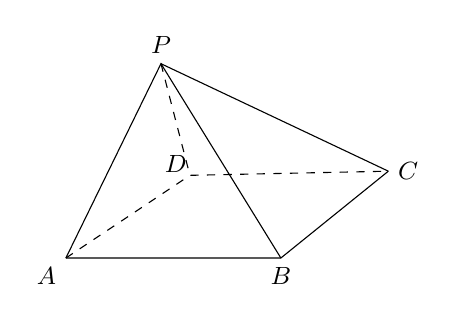
\begin{tikzpicture}[scale=1.05, font=\small]
  \coordinate (P) at (1.15,2.35);
  \coordinate (A) at (0,0);
  \coordinate (B) at (2.6,0);
  \coordinate (C) at (3.9,1.05);
  \coordinate (D) at (1.5,1.0);
  \draw (A) -- (B) -- (C);
  \draw (A) -- (P) -- (B);
  \draw (P) -- (C);
  \draw[dashed] (A) -- (D) -- (C);
  \draw[dashed] (P) -- (D);
  \node[above] at (P) {$P$};
  \node[below left] at (A) {$A$};
  \node[below] at (B) {$B$};
  \node[right] at (C) {$C$};
  \node[above left, inner sep=1pt] at (D) {$D$};
\end{tikzpicture}
\end{center}
\nopagebreak[4]
  (1) 证明：平面 $PAB\perp$ 平面 $PAD$；

  (2) 若 $PA=PD=AB=DC$，$\angle APD=90^\circ$，且四棱锥 $P\text{-}ABCD$ 的体积为 $\dfrac83$，求该四棱锥的侧面积。

\Needspace{4\baselineskip}
\textbf{解析}

\gksubpart{(1) 证明平面 $PAB\perp$ 平面 $PAD$}

（同理科卷第 18(1) 题）

\Needspace{5\baselineskip}
由 $\angle BAP=90^\circ$ 得 $AB\perp AP$；由 $\angle CDP=90^\circ$ 得 $CD\perp PD$，而 $AB\parallel CD$，故

\nopagebreak[4]
\[AB\perp PD\]

\Needspace{5\baselineskip}
$AP$ 与 $PD$ 是平面 $PAD$ 内的两条相交直线（交于 $P$），由线面垂直判定定理：

\nopagebreak[4]
\[AB\perp\text{\text{平面} }PAD\]

\Needspace{5\baselineskip}
又 $AB\subset$ 平面 $PAB$，故

\nopagebreak[4]
\[\text{\text{平面} }PAB\perp\text{\text{平面} }PAD\qquad\blacksquare\]

\gksubpart{(2) 求四棱锥的侧面积}

设 $PA=PD=AB=DC=2a\ (a>0)$。

\textbf{第一步：认清底面形状。} 由 (1)，$AB\perp$ 平面 $PAD$，故 $AB\perp AD$。又 $AB\parallel CD$ 且 $AB=CD$，所以 $ABCD$ 是平行四边形，再加上 $AB\perp AD$，它是\textbf{矩形}。

\Needspace{5\baselineskip}
由 $\angle APD=90^\circ$、$PA=PD=2a$ 得

\nopagebreak[4]
\[AD=\sqrt{(2a)^{2}+(2a)^{2}}=2\sqrt2a\]

\textbf{第二步：用体积定出 $a$。}

\Needspace{5\baselineskip}
底面积：

\nopagebreak[4]
\[S_{ABCD}=AB\times AD=2a\times2\sqrt2a=4\sqrt2a^{2}\]

\Needspace{5\baselineskip}
高：因 $AB\perp$ 平面 $PAD$，平面 $PAD\perp$ 底面，$P$ 到底面的距离等于 $P$ 到 $AD$ 的距离，即等腰直角三角形 $PAD$ 斜边上的高：

\nopagebreak[4]
\[h=\frac{PA\cdot PD}{AD}=\frac{4a^{2}}{2\sqrt2a}=\sqrt2a\]

\nopagebreak[4]
\[V=\frac13\times4\sqrt2a^{2}\times\sqrt2a=\frac13\times8a^{3}=\frac{8a^{3}}3\]

\Needspace{5\baselineskip}
由 $V=\dfrac83$：

\nopagebreak[4]
\[a^{3}=1\ \Longrightarrow\ a=1\]

\Needspace{5\baselineskip}
所以

\nopagebreak[4]
\[PA=PD=AB=DC=2,\qquad AD=BC=2\sqrt2\]

\textbf{第三步：逐个算四个侧面的面积。}

\begin{itemize}
\item \textbf{$\triangle PAD$}：直角边 $PA=PD=2$，$\angle APD=90^\circ$，
\end{itemize}
\nopagebreak[4]
\[S=\frac12\times2\times2=2\]
\begin{itemize}
\item \textbf{$\triangle PAB$}：由 $AB\perp$ 平面 $PAD$ 知 $AB\perp PA$，是直角三角形，直角边 $PA=2$、$AB=2$，
\end{itemize}
\nopagebreak[4]
\[S=\frac12\times2\times2=2\]
\begin{itemize}
\item \textbf{$\triangle PDC$}：由 $\angle CDP=90^\circ$，直角边 $PD=2$、$DC=2$，
\end{itemize}
\nopagebreak[4]
\[S=\frac12\times2\times2=2\]
\begin{itemize}
\item \textbf{$\triangle PBC$}：需要三边。建系计算最稳妥 —— 以 $A$ 为原点、$AD$ 为 $x$ 轴、$AB$ 为 $y$ 轴、竖直向上为 $z$ 轴：
\end{itemize}
\nopagebreak[4]
\[A(0,0,0),\quad D\left(2\sqrt2,0,0\right),\quad B(0,2,0),\quad C\left(2\sqrt2,2,0\right),\quad P\left(\sqrt2,0,\sqrt2\right)\]
\nopagebreak[4]
\[PB=\sqrt{2+4+2}=2\sqrt2,\qquad PC=\sqrt{\left(2\sqrt2-\sqrt2\right)^{2}+4+2}=\sqrt{2+4+2}=2\sqrt2\]
\nopagebreak[4]
\[BC=2\sqrt2\]
\Needspace{5\baselineskip}
  三边相等，是\textbf{边长为 $2\sqrt2$ 的等边三角形}：
\nopagebreak[4]
\[S=\frac{\sqrt3}4\times\left(2\sqrt2\right)^{2}=\frac{\sqrt3}4\times8=2\sqrt3\]

\Needspace{5\baselineskip}
\textbf{第四步：求和。}

\nopagebreak[4]
\[S_{\text{\text{侧}}}=2+2+2+2\sqrt3=6+2\sqrt3\]

\begin{gktip}
\textbf{方法提示}：求侧面积必须\textbf{逐个面判断形状}，不能想当然。本题三个侧面是直角三角形（由题设的两个直角和 (1) 的结论直接得到），第四个 $\triangle PBC$ 恰好是等边三角形 —— 这个"意外"只有算出三边才能发现，所以建系算坐标是最可靠的路。

另外注意区分"侧面积"（四个侧面）与"表面积"（还要加底面）。
\end{gktip}

\gkanswer{答案（1）：见解析版}

\gkanswer{答案（2）：侧面积 $=6+2\sqrt3$}

\par\medskip

\end{answer}
\begin{answer}
\gksolhead{19}{12 分，相关系数与质量监控}

\textbf{题目}（12 分）：

为了监控某种零件的一条生产线的生产过程，检验员每隔 $30\ \min$ 从该生产线上随机抽取一个零件，并测量其尺寸（单位：$\mathrm{cm}$）。下面是检验员在一天内依次抽取的 $16$ 个零件的尺寸：

\begin{center}
\begingroup\setlength{\tabcolsep}{4pt}
\begin{tabular}{ccccccccc}
\toprule
抽取次序 & $1$ & $2$ & $3$ & $4$ & $5$ & $6$ & $7$ & $8$ \\
\midrule
零件尺寸 & $9.95$ & $10.12$ & $9.96$ & $9.96$ & $10.01$ & $9.92$ & $9.98$ & $10.04$ \\
\bottomrule
\end{tabular}
\endgroup
\end{center}

\begin{center}
\begingroup\setlength{\tabcolsep}{4pt}
\begin{tabular}{ccccccccc}
\toprule
抽取次序 & $9$ & $10$ & $11$ & $12$ & $13$ & $14$ & $15$ & $16$ \\
\midrule
零件尺寸 & $10.26$ & $9.91$ & $10.13$ & $10.02$ & $9.22$ & $10.04$ & $10.05$ & $9.95$ \\
\bottomrule
\end{tabular}
\endgroup
\end{center}

\Needspace{5\baselineskip}
经计算得

\nopagebreak[4]
\[\bar x=\frac1{16}\sum_{i=1}^{16}x_i=9.97,\qquad s=\sqrt{\frac1{16}\sum_{i=1}^{16}\left(x_i-\bar x\right)^{2}}=\sqrt{\frac1{16}\left(\sum_{i=1}^{16}x_i^{2}-16\bar x^{2}\right)}\approx0.212\]

\nopagebreak[4]
\[\sqrt{\sum_{i=1}^{16}(i-8.5)^{2}}\approx18.439,\qquad \sum_{i=1}^{16}\left(x_i-\bar x\right)(i-8.5)=-2.78\]

其中 $x_i$ 为抽取的第 $i$ 个零件的尺寸，$i=1,2,\cdots,16$。

  (1) 求 $\left(x_i,\ i\right)\ (i=1,2,\cdots,16)$ 的相关系数 $r$，并回答是否可以认为这一天生产的零件尺寸不随生产过程的进行而系统地变大或变小（若 $|r|<0.25$，则可以认为零件的尺寸不随生产过程的进行而系统地变大或变小）；

  (2) 一天内抽检零件中，如果出现了尺寸在 $(\bar x-3s,\ \bar x+3s)$ 之外的零件，就认为这条生产线在这一天的生产过程可能出现了异常情况，需对当天的生产过程进行检查。

  　① 从这一天抽检的结果看，是否需对当天的生产过程进行检查？

  　② 在 $(\bar x-3s,\ \bar x+3s)$ 之外的数据称为离群值，试剔除离群值，估计这条生产线当天生产的零件尺寸的均值与标准差（精确到 $0.01$）。

\Needspace{5\baselineskip}
  附：样本 $\left(x_i,y_i\right)\ (i=1,2,\cdots,n)$ 的相关系数

\nopagebreak[4]
\[r=\frac{\sum\limits_{i=1}^{n}\left(x_i-\bar x\right)\left(y_i-\bar y\right)}{\sqrt{\sum\limits_{i=1}^{n}\left(x_i-\bar x\right)^{2}}\sqrt{\sum\limits_{i=1}^{n}\left(y_i-\bar y\right)^{2}}},\qquad \sqrt{0.008}\approx0.09\]

\Needspace{4\baselineskip}
\textbf{解析}

\gksubpart{(1) 求相关系数 $r$ 并作判断}

\Needspace{5\baselineskip}
\textbf{明确两个变量}：$x_i$ 是零件尺寸，$i$ 是抽取次序（$i=1,2,\cdots,16$）。

\nopagebreak[4]
\[\bar i=\frac{1+2+\cdots+16}{16}=\frac{136}{16}=8.5\]

（这正是题目中出现 $i-8.5$ 的原因。）

\textbf{分母的两个因子}：

\begin{itemize}
\item 由 $s=\sqrt{\dfrac1{16}\sum\left(x_i-\bar x\right)^{2}}\approx0.212$ 反推
\end{itemize}
\nopagebreak[4]
\[\sqrt{\sum_{i=1}^{16}\left(x_i-\bar x\right)^{2}}=4s=4\times0.212=0.848\]
\begin{itemize}
\item 题目直接给出
\end{itemize}
\nopagebreak[4]
\[\sqrt{\sum_{i=1}^{16}(i-8.5)^{2}}\approx18.439\]

\Needspace{5\baselineskip}
\textbf{代入公式}：

\nopagebreak[4]
\[r=\frac{\sum\limits_{i=1}^{16}\left(x_i-\bar x\right)(i-8.5)}{\sqrt{\sum\left(x_i-\bar x\right)^{2}}\cdot\sqrt{\sum(i-8.5)^{2}}}=\frac{-2.78}{0.848\times18.439}=\frac{-2.78}{15.636}\approx-0.18\]

\Needspace{5\baselineskip}
\textbf{作判断}：

\nopagebreak[4]
\[|r|=0.18<0.25\]

\textbf{结论：可以认为这一天生产的零件尺寸不随生产过程的进行而系统地变大或变小。}

\gksubpart{(2) ① 是否需要检查}

\nopagebreak[4]
\[3s=3\times0.212=0.636\]

\nopagebreak[4]
\[(\bar x-3s,\ \bar x+3s)=(9.97-0.636,\ 9.97+0.636)=(9.334,\ 10.606)\]

\Needspace{5\baselineskip}
逐个核对 $16$ 个数据，发现第 $13$ 个数据

\nopagebreak[4]
\[x_{13}=9.22<9.334\]

落在区间之外（其余 $15$ 个都在区间内）。

\textbf{结论：需要对当天的生产过程进行检查。}

\gksubpart{(2) ② 剔除离群值后重新估计}

离群值就是 $9.22$，剔除后剩 $15$ 个数据。

\Needspace{5\baselineskip}
\textbf{新均值}：

\nopagebreak[4]
\[\bar x'=\frac{16\bar x-9.22}{15}=\frac{16\times9.97-9.22}{15}=\frac{159.52-9.22}{15}=\frac{150.30}{15}=10.02\]

\Needspace{5\baselineskip}
\textbf{新标准差}：先由 $s$ 反推原来的平方和：

\nopagebreak[4]
\[\sum_{i=1}^{16}x_i^{2}=16s^{2}+16\bar x^{2}=16\times0.212^{2}+16\times9.97^{2}\approx0.7191+1590.4144=1591.1335\]

\Needspace{5\baselineskip}
剔除 $9.22$：

\nopagebreak[4]
\[\sum{}'x_i^{2}=1591.1335-9.22^{2}=1591.1335-85.0084=1506.1251\]

\nopagebreak[4]
\[s'^{2}=\frac1{15}\left(\sum{}'x_i^{2}-15\bar x'^{2}\right)=\frac{1506.1251-15\times10.02^{2}}{15}\]

\nopagebreak[4]
\[=\frac{1506.1251-1506.0060}{15}\approx0.008\]

\nopagebreak[4]
\[s'=\sqrt{0.008}\approx0.09\]

\begin{gktip}
\textbf{方法提示}：本题两个小问的结论看似矛盾（"没有系统趋势"却"需要检查"），其实正是统计学要传达的意思：

\begin{itemize}
\item \textbf{相关系数}检验的是"\textbf{有没有随时间单调漂移的趋势}"—— 答案是没有；
\item \textbf{$3\sigma$ 准则}检验的是"\textbf{有没有个别离群的异常点}"—— 答案是有一个。
\end{itemize}

两种检验回答的是不同的问题，一个生产过程完全可能"没有系统漂移但出了一次意外"。

计算上的两个要点：$\sqrt{\sum\left(x_i-\bar x\right)^{2}}=4s$（因为样本量是 $16$，$\sqrt{16}=4$）；以及用"\textbf{平方和减 $n$ 倍均值平方}"算新的标准差，比逐个求差快得多。题干把 $s$ 写成两种等价形式，正是在提示这条路。
\end{gktip}

\gkanswer{答案（1）：$r\approx-0.18$；可以认为尺寸不随生产过程系统地变大或变小}

\gkanswer{答案（2）：① 需要检查；② 均值 $10.02$，标准差约 $0.09$}

\par\medskip

\end{answer}
\begin{answer}
\gksolhead{20}{12 分，抛物线}

\textbf{题目}（12 分）：

设 $A$，$B$ 为曲线 $C:y=\dfrac{x^{2}}4$ 上两点，$A$ 与 $B$ 的横坐标之和为 $4$。

  (1) 求直线 $AB$ 的斜率；

  (2) 设 $M$ 为曲线 $C$ 上一点，$C$ 在 $M$ 处的切线与直线 $AB$ 平行，且 $AM\perp BM$，求直线 $AB$ 的方程。

\Needspace{4\baselineskip}
\textbf{解析}

\gksubpart{(1) 求直线 $AB$ 的斜率}

\Needspace{5\baselineskip}
设 $A\left(x_1,\dfrac{x_1^{2}}4\right)$，$B\left(x_2,\dfrac{x_2^{2}}4\right)$，$x_1\ne x_2$，且 $x_1+x_2=4$。

\nopagebreak[4]
\[k=\frac{\frac{x_2^{2}}4-\frac{x_1^{2}}4}{x_2-x_1}=\frac{x_2^{2}-x_1^{2}}{4\left(x_2-x_1\right)}=\frac{\left(x_2-x_1\right)\left(x_2+x_1\right)}{4\left(x_2-x_1\right)}=\frac{x_1+x_2}4=\frac44=1\]

\begin{gktip}
这就是抛物线的"\textbf{点差法}"：割线斜率只与两点横坐标之和有关。
\end{gktip}

\gksubpart{(2) 求直线 $AB$ 的方程}

\Needspace{5\baselineskip}
\textbf{第一步：定出 $M$。} 由 $y=\dfrac{x^{2}}4$ 得 $y'=\dfrac x2$。切线与 $AB$ 平行即斜率为 $1$：

\nopagebreak[4]
\[\frac{x_M}2=1\ \Longrightarrow\ x_M=2,\qquad y_M=\frac{2^{2}}4=1\]

\nopagebreak[4]
\[M(2,1)\]

\Needspace{5\baselineskip}
\textbf{第二步：设 $AB$ 并联立。} 由 (1) 知斜率为 $1$，设

\nopagebreak[4]
\[AB:\ y=x+m\]

\Needspace{5\baselineskip}
代入抛物线：

\nopagebreak[4]
\[\frac{x^{2}}4=x+m\ \Longrightarrow\ x^{2}-4x-4m=0\]

\Needspace{5\baselineskip}
韦达定理：

\nopagebreak[4]
\[x_1+x_2=4\ (\text{\text{与题设一致，自动满足}}),\qquad x_1x_2=-4m\]

\Needspace{5\baselineskip}
两点相异要求判别式为正：

\nopagebreak[4]
\[\Delta=16+16m>0\ \Longrightarrow\ m>-1\]

\Needspace{5\baselineskip}
\textbf{第三步：用 $AM\perp BM$ 列方程。}

\nopagebreak[4]
\[\overrightarrow{MA}=\left(x_1-2,\ \frac{x_1^{2}}4-1\right),\qquad \overrightarrow{MB}=\left(x_2-2,\ \frac{x_2^{2}}4-1\right)\]

\Needspace{5\baselineskip}
\textbf{关键的因式分解}：

\nopagebreak[4]
\[\frac{x^{2}}4-1=\frac{x^{2}-4}4=\frac{(x-2)(x+2)}4\]

\Needspace{5\baselineskip}
于是

\nopagebreak[4]
\[\overrightarrow{MA}\cdot\overrightarrow{MB}=\left(x_1-2\right)\left(x_2-2\right)+\frac{\left(x_1-2\right)\left(x_1+2\right)\left(x_2-2\right)\left(x_2+2\right)}{16}\]

\Needspace{5\baselineskip}
提取公因式 $\left(x_1-2\right)\left(x_2-2\right)$：

\nopagebreak[4]
\[=\left(x_1-2\right)\left(x_2-2\right)\left[1+\frac{\left(x_1+2\right)\left(x_2+2\right)}{16}\right]=0\]

\Needspace{5\baselineskip}
\textbf{第四步：判断哪个因子为零。}

\nopagebreak[4]
\[\left(x_1-2\right)\left(x_2-2\right)=x_1x_2-2\left(x_1+x_2\right)+4=-4m-8+4=-4(m+1)\]

\Needspace{5\baselineskip}
由 $m>-1$ 知 $-4(m+1)\ne0$，故\textbf{第一个因子非零}，必须

\nopagebreak[4]
\[1+\frac{\left(x_1+2\right)\left(x_2+2\right)}{16}=0\]

\Needspace{5\baselineskip}
计算：

\nopagebreak[4]
\[\left(x_1+2\right)\left(x_2+2\right)=x_1x_2+2\left(x_1+x_2\right)+4=-4m+8+4=12-4m\]

\Needspace{5\baselineskip}
代入：

\nopagebreak[4]
\[1+\frac{12-4m}{16}=0\ \Longrightarrow\ 16+12-4m=0\ \Longrightarrow\ m=7\]

\textbf{检验}：$m=7>-1$  判别式为正，$A$、$B$ 确实存在。

\begin{gktip}
\textbf{方法提示}：本题第 (2) 问的漂亮之处在于\textbf{把 $\dfrac{x^{2}}4-1$ 分解出 $(x-2)$ 这个公因子}（$2$ 正是切点 $M$ 的横坐标），使得数量积能提取公因式，从而把一个看似复杂的方程拆成"两个因子之一为零"。

提取后一定要\textbf{说明第一个因子不为零}（用判别式条件 $m>-1$），否则逻辑不完整 —— 若 $\left(x_1-2\right)\left(x_2-2\right)=0$，意味着 $A$ 或 $B$ 与 $M$ 重合，$AM\perp BM$ 本就无从谈起。
\end{gktip}

\gkanswer{答案（1）：$k=1$}

\gkanswer{答案（2）：$y=x+7$}

\par\medskip

\end{answer}
\begin{answer}
\gksolhead{21}{12 分，导数}

\textbf{题目}（12 分）：

已知函数 $f(x)=\mathrm e^{x}\left(\mathrm e^{x}-a\right)-a^{2}x$。

  (1) 讨论 $f(x)$ 的单调性；

  (2) 若 $f(x)\ge0$，求 $a$ 的取值范围。

\Needspace{4\baselineskip}
\textbf{解析}

\gksubpart{(1) 讨论 $f(x)$ 的单调性}

\nopagebreak[4]
\[f'(x)=2\mathrm e^{2x}-a\mathrm e^{x}-a^{2}\]

\Needspace{5\baselineskip}
\textbf{因式分解}（把它看作关于 $\mathrm e^{x}$ 的二次三项式）：

\nopagebreak[4]
\[\left(2\mathrm e^{x}+a\right)\left(\mathrm e^{x}-a\right)=2\mathrm e^{2x}-2a\mathrm e^{x}+a\mathrm e^{x}-a^{2}=2\mathrm e^{2x}-a\mathrm e^{x}-a^{2}\ \checkmark\]

\Needspace{5\baselineskip}
所以

\nopagebreak[4]
\[f'(x)=\left(2\mathrm e^{x}+a\right)\left(\mathrm e^{x}-a\right)\]

\textbf{分三种情况讨论：}

\Needspace{5\baselineskip}
\textbf{情形一：$a=0$。}

\nopagebreak[4]
\[f'(x)=2\mathrm e^{2x}>0\]

$f(x)$ 在 $(-\infty,+\infty)$ 上\textbf{单调递增}。

\textbf{情形二：$a>0$。}

\Needspace{5\baselineskip}
此时 $2\mathrm e^{x}+a>0$ 恒成立，符号由第二个因子决定：

\nopagebreak[4]
\[\mathrm e^{x}-a>0\iff x>\ln a\]

\begin{itemize}
\item $f(x)$ 在 $(-\infty,\ln a)$ 上\textbf{单调递减}；
\item $f(x)$ 在 $(\ln a,+\infty)$ 上\textbf{单调递增}。
\end{itemize}

\textbf{情形三：$a<0$。}

\Needspace{5\baselineskip}
此时 $\mathrm e^{x}-a>0$ 恒成立（因 $-a>0$），符号由第一个因子决定：

\nopagebreak[4]
\[2\mathrm e^{x}+a>0\iff \mathrm e^{x}>-\frac a2\iff x>\ln\left(-\frac a2\right)\]

\begin{itemize}
\item $f(x)$ 在 $\left(-\infty,\ \ln\left(-\dfrac a2\right)\right)$ 上\textbf{单调递减}；
\item $f(x)$ 在 $\left(\ln\left(-\dfrac a2\right),\ +\infty\right)$ 上\textbf{单调递增}。
\end{itemize}

\gksubpart{(2) 若 $f(x)\ge0$，求 $a$ 的取值范围}

按 (1) 的三种情形分别求最小值。

\Needspace{5\baselineskip}
\textbf{情形一：$a=0$。}

\nopagebreak[4]
\[f(x)=\mathrm e^{2x}>0\ \checkmark\]

恒成立，$a=0$ 可取。

\Needspace{5\baselineskip}
\textbf{情形二：$a>0$。} 最小值在 $x=\ln a$ 处，此时 $\mathrm e^{x}=a$：

\nopagebreak[4]
\[f(\ln a)=a^{2}-a\cdot a-a^{2}\ln a=-a^{2}\ln a\]

\Needspace{5\baselineskip}
要求

\nopagebreak[4]
\[-a^{2}\ln a\ge0\ \Longrightarrow\ \ln a\le0\ \Longrightarrow\ a\le1\]

\Needspace{5\baselineskip}
结合 $a>0$：

\nopagebreak[4]
\[0<a\le1\]

\Needspace{5\baselineskip}
\textbf{情形三：$a<0$。} 最小值在 $x_0=\ln\left(-\dfrac a2\right)$ 处，此时 $\mathrm e^{x_0}=-\dfrac a2$：

\nopagebreak[4]
\[f\left(x_0\right)=\left(-\frac a2\right)^{2}-a\left(-\frac a2\right)-a^{2}\ln\left(-\frac a2\right)=\frac{a^{2}}4+\frac{a^{2}}2-a^{2}\ln\left(-\frac a2\right)\]

\nopagebreak[4]
\[=a^{2}\left[\frac34-\ln\left(-\frac a2\right)\right]\]

\Needspace{5\baselineskip}
因 $a^{2}>0$，要求

\nopagebreak[4]
\[\frac34-\ln\left(-\frac a2\right)\ge0\ \Longrightarrow\ \ln\left(-\frac a2\right)\le\frac34\ \Longrightarrow\ -\frac a2\le\mathrm e^{3/4}\ \Longrightarrow\ a\ge-2\mathrm e^{3/4}\]

\Needspace{5\baselineskip}
结合 $a<0$：

\nopagebreak[4]
\[-2\mathrm e^{3/4}\le a<0\]

\Needspace{5\baselineskip}
\textbf{三种情形合并}：

\nopagebreak[4]
\[a\in\left[-2\mathrm e^{3/4},\ 1\right]\]

\begin{gktip}
\textbf{方法提示}：本题的三个要点：

1. \textbf{$f'$ 的因式分解}是全题的钥匙。$2\mathrm e^{2x}-a\mathrm e^{x}-a^{2}$ 视作 $2t^{2}-at-a^{2}$（$t=\mathrm e^{x}$），分解为 $(2t+a)(t-a)$。
2. \textbf{按 $a$ 的符号分三类讨论}，因为哪个因子起决定作用取决于 $a$ 的正负 —— 这是最容易漏掉情形的地方（很多人只讨论 $a>0$ 和 $a\le0$ 两类，会把 $a=0$ 的退化情形与 $a<0$ 混在一起）。
3. \textbf{恒成立 $\iff$ 最小值 $\ge0$}，最小值处 $\mathrm e^{x_0}$ 的值已由 (1) 给出，代入时直接换掉指数即可，不必写成含 $\ln$ 的复杂式子。
\end{gktip}

\gkanswer{答案（1）：$f'(x)=\left(2\mathrm e^{x}+a\right)\left(\mathrm e^{x}-a\right)$。$a=0$：在 $\mathbf R$ 上单调递增；$a>0$：在 $(-\infty,\ln a)$ 递减、$(\ln a,+\infty)$ 递增；$a<0$：在 $\left(-\infty,\ln\left(-\dfrac a2\right)\right)$ 递减、$\left(\ln\left(-\dfrac a2\right),+\infty\right)$ 递增。}

\gkanswer{答案（2）：$-2\mathrm e^{3/4}\le a\le1$}

\par\medskip

\end{answer}
\gkpart{选考题（现行考纲已取消，仅存档）}

\begin{answer}
\gksolhead{22}{10 分，坐标系与参数方程}

\textbf{题目}（10 分）〔选修 4-4：坐标系与参数方程〕：

（\textbf{已取消}）

在直角坐标系 $xOy$ 中，曲线 $C$ 的参数方程为 $\begin{cases}x=3\cos\theta\\ y=\sin\theta\end{cases}$（$\theta$ 为参数），直线 $l$ 的参数方程为 $\begin{cases}x=a+4t\\ y=1-t\end{cases}$（$t$ 为参数）。

  (1) 若 $a=-1$，求 $C$ 与 $l$ 的交点坐标；

  (2) 若 $C$ 上的点到 $l$ 距离的最大值为 $\sqrt{17}$，求 $a$。

\textbf{解析}（同理科卷第 22 题）

\gksubpart{(1) $a=-1$ 时的交点}

$C$ 的普通方程：$\dfrac{x^{2}}9+y^{2}=1$。

$l$ 消参（$t=1-y$）：$x=-1+4(1-y)$，即 $x+4y-3=0$。

\Needspace{5\baselineskip}
联立（把 $x=3-4y$ 代入）：

\nopagebreak[4]
\[(3-4y)^{2}+9y^{2}=9\ \Longrightarrow\ 25y^{2}-24y=0\ \Longrightarrow\ y=0\ \text{\text{或}}\ y=\frac{24}{25}\]

\Needspace{5\baselineskip}
对应交点：

\nopagebreak[4]
\[(3,\ 0)\qquad\text{\text{与}}\qquad\left(-\frac{21}{25},\ \frac{24}{25}\right)\]

\gksubpart{(2) 最大距离为 $\sqrt{17}$ 时求 $a$}

\Needspace{5\baselineskip}
一般的 $l$：$x+4y-a-4=0$。设 $C$ 上的点为 $(3\cos\theta,\sin\theta)$：

\nopagebreak[4]
\[d=\frac{|3\cos\theta+4\sin\theta-a-4|}{\sqrt{17}}=\frac{\left|5\sin(\theta+\varphi)-a-4\right|}{\sqrt{17}}\]

\Needspace{5\baselineskip}
其中 $5\sin(\theta+\varphi)\in[-5,5]$。最大值在端点取到：

\nopagebreak[4]
\[d_{\max}=\frac{\max\{|1-a|,\ |a+9|\}}{\sqrt{17}}=\sqrt{17}\ \Longrightarrow\ \max\{|1-a|,\ |a+9|\}=17\]

\begin{itemize}
\item $a=8$：$|1-8|=7$，$|8+9|=17$，最大值 $17$ 
\item $a=-16$：$|1+16|=17$，$|-16+9|=7$，最大值 $17$ 
\item $a=-26$ 与 $a=18$：另一项达到 $27>17$，\textbf{舍去}。
\end{itemize}

\gkanswer{答案（1）：$(3,0)$ 与 $\left(-\dfrac{21}{25},\dfrac{24}{25}\right)$}

\gkanswer{答案（2）：$a=8$ 或 $a=-16$}

\par\medskip

\end{answer}
\begin{answer}
\gksolhead{23}{10 分，不等式选讲}

\textbf{题目}（10 分）〔选修 4-5：不等式选讲〕：

（\textbf{已取消}）

已知函数 $f(x)=-x^{2}+ax+4$，$g(x)=|x+1|+|x-1|$。

  (1) 当 $a=1$ 时，求不等式 $f(x)\ge g(x)$ 的解集；

  (2) 若不等式 $f(x)\ge g(x)$ 的解集包含 $[-1,1]$，求 $a$ 的取值范围。

\par\medskip

\textbf{解析}（同理科卷第 23 题）

\gksubpart{(1) $a=1$ 时解 $f(x)\ge g(x)$}

分三段去绝对值：

\begin{itemize}
\item \textbf{$x<-1$}：$g=-2x$，不等式化为 $x^{2}-3x-4\le0$，解得 $-1\le x\le4$，与本段\textbf{无交集}；
\item \textbf{$-1\le x\le1$}：$g=2$，不等式化为 $x^{2}-x-2\le0$，解得 $-1\le x\le2$，本段\textbf{全部满足}；
\item \textbf{$x>1$}：$g=2x$，不等式化为 $x^{2}+x-4\le0$，解得 $x\le\dfrac{\sqrt{17}-1}2\approx1.56$，交得 $1<x\le\dfrac{\sqrt{17}-1}2$。
\end{itemize}

\gksubpart{(2) 解集包含 $[-1,1]$ 时求 $a$}

\Needspace{5\baselineskip}
在 $[-1,1]$ 上 $g(x)\equiv2$，条件化为

\nopagebreak[4]
\[-x^{2}+ax+4\ge2\iff ax\ge x^{2}-2\quad\text{\text{对一切}}\ x\in[-1,1]\]

按 $x$ 的符号分离参数（记 $h(x)=x-\dfrac2x$，它在 $(0,1]$ 与 $[-1,0)$ 上都单调递增）：

\begin{itemize}
\item $x=0$：$0\ge-2$ 恒成立；
\item $x\in(0,1]$：$a\ge h(x)$，最大值 $h(1)=-1$，故 $a\ge-1$；
\item $x\in[-1,0)$：除以负数变号，$a\le h(x)$，最小值 $h(-1)=1$，故 $a\le1$。
\end{itemize}

\par\medskip

\gkanswer{答案（1）：$\left[-1,\dfrac{\sqrt{17}-1}2\right]$}

\gkanswer{答案（2）：$-1\le a\le1$}

\end{answer}